\documentclass{cshwk}
\begin{document}
\title{Wireshark Lab \#1, Intro}
\maketitle

\section*{Problem 1.Protocols}
\begin{quote}
    List 3 different protocols that appear in the protocol column in the unfiltered packet-listing window in step 7 above.
\end{quote}

\subsection*{Solves:}
\begin{figure}[htbp]
    \centering
    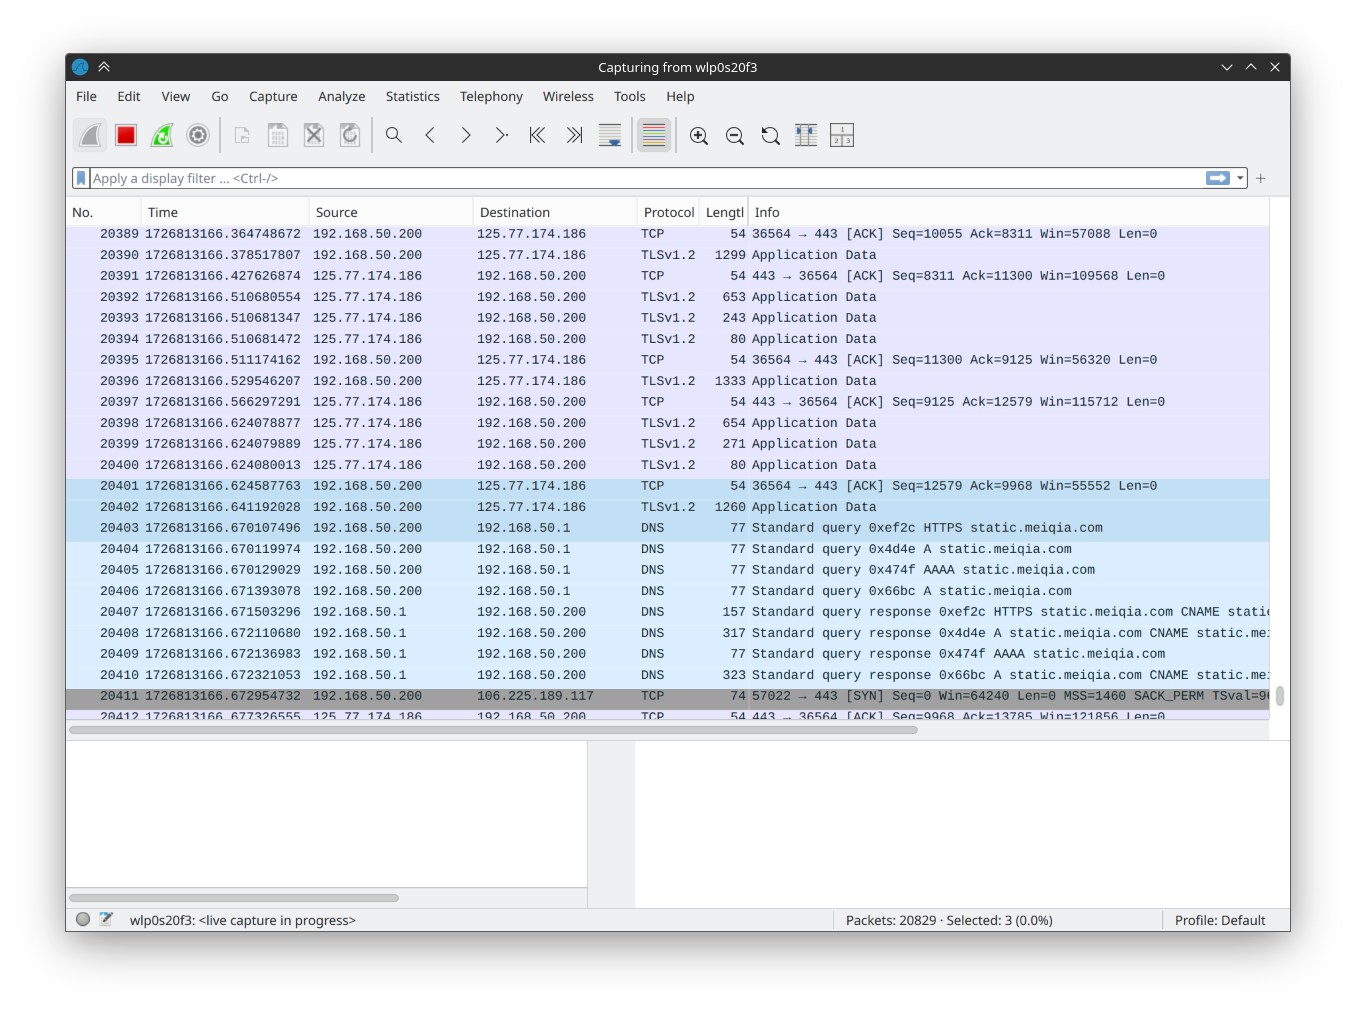
\includegraphics[width=0.8\textwidth]{./lab1-1.png}
    \caption{The protocol column in the unfiltered packet-listing window}
    \label{fig:protocols}
\end{figure}
Open Wireshark and wait for the packet sniffer to start. The three protocols that appear in the protocol column are
\begin{enumerate}
    \item DNS
    \item HTTP
    \item TLSv1.2
\end{enumerate}
The details are showned in the Fig.~\ref{fig:protocols}:

\section*{Problem 2. Request Timing}
\begin{quote}
    How long did it take from when the HTTP GET message was sent until the HTTP OK reply was received? (By default, the value of the Time column in the packet-listing window is the amount of time, in seconds, since Wireshark tracing began. To display the Time field in time-of-day format, select the Wireshark View pull down menu, then select Time Display Format, then select Time-of-day.)
\end{quote}

\subsection*{Solves:}

I used the Linux command \texttt{curl} to send a simple HTTP request and observed the updates in Wireshark.
\begin{verbatim}
    curl www.baidu.com
\end{verbatim}
\begin{figure}[htbp]
    \centering
    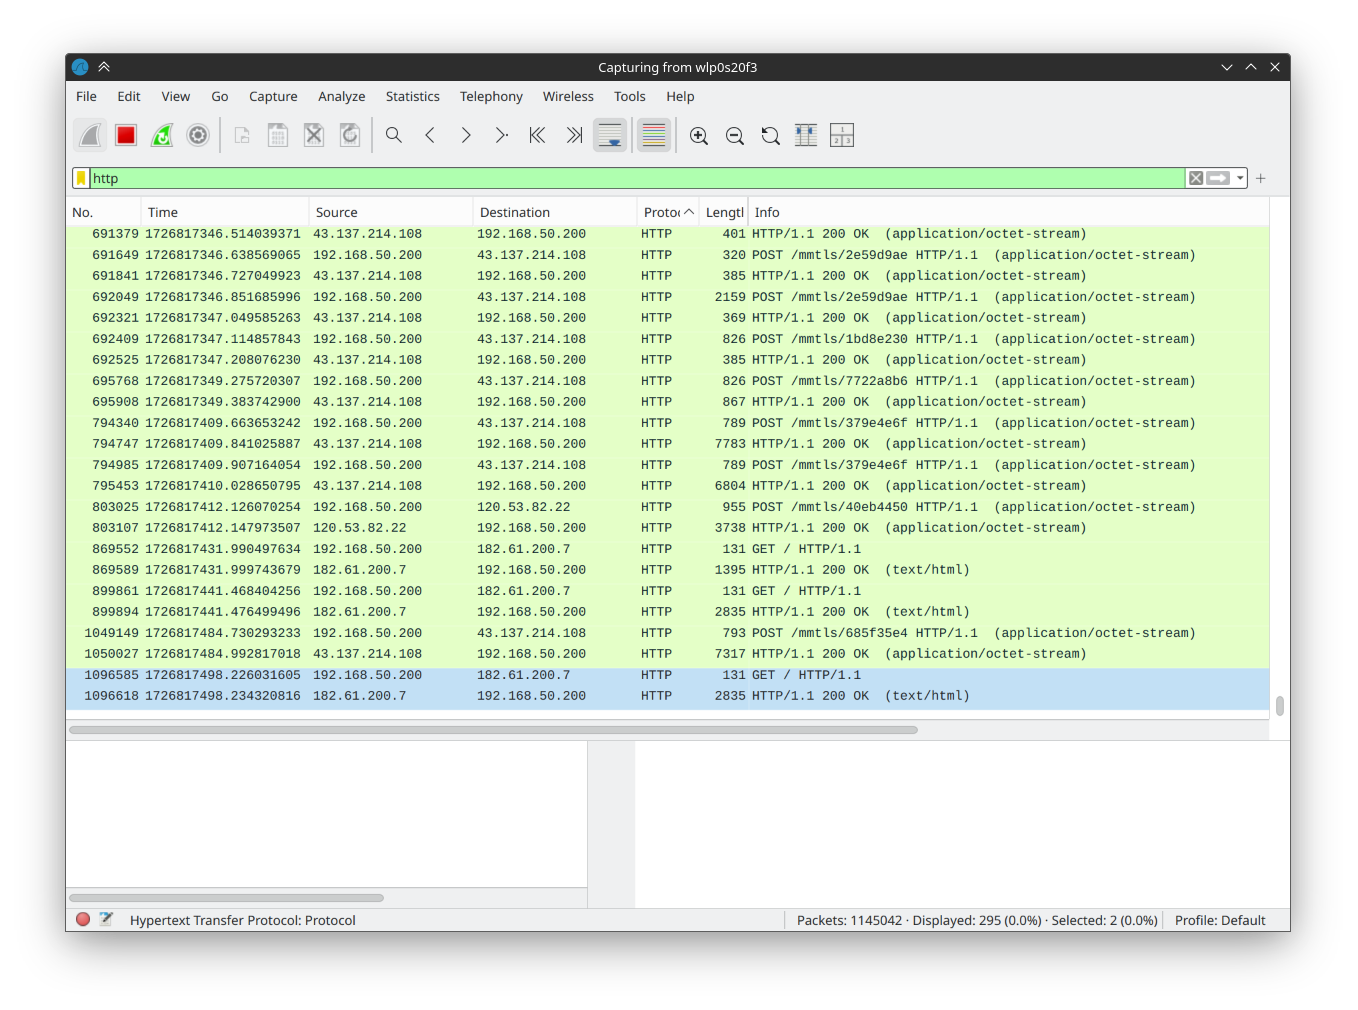
\includegraphics[width=0.8\textwidth]{./lab1-2.png}
    \caption{The time from HTTP GET to HTTP OK}
    \label{fig:timing}
\end{figure}

There are two rows in the packet-listing window: one represents the HTTP GET request, and the other shows the HTTP OK reply. By observing the time column for these two rows, we can measure the time difference, which is the duration from the HTTP GET to HTTP OK response. The result is shown in Fig.~\ref{fig:timing}.

The time column displays the timestamp of each packet, based on the configured settings. It represents the total number of seconds since 1970-01-01 00:00:00 UTC.

Therefore, the time from HTTP GET to HTTP OK can be calculated as:
\begin{align*}
    t_{GET-OK} & = t_{OK} - t_{GET}                                                  \\
               & = 1726817498.234320816~\mathbf{s} - 1726817498.226031605~\mathbf{s} \\
               & \boxed{= 0.008289211 ~\mathbf{s}}
\end{align*}

\section*{Problem 3. Internet Address}

\begin{quote}
    What is the Internet address of the \href{http://gaia.cs.umass.edu}{gaia.cs.umass.edu} \\
    (also known as \href{http://www-net.cs.umass.edu}{www-net.cs.umass.edu})?\\
    What is the Internet address of your computer?
\end{quote}

\subsection*{Solves:}
Also, use the \texttt{curl} command to send a simple HTTP request:
\begin{verbatim}
    curl gaia.cs.umass.edu
\end{verbatim}

\begin{figure}[htbp]
    \centering
    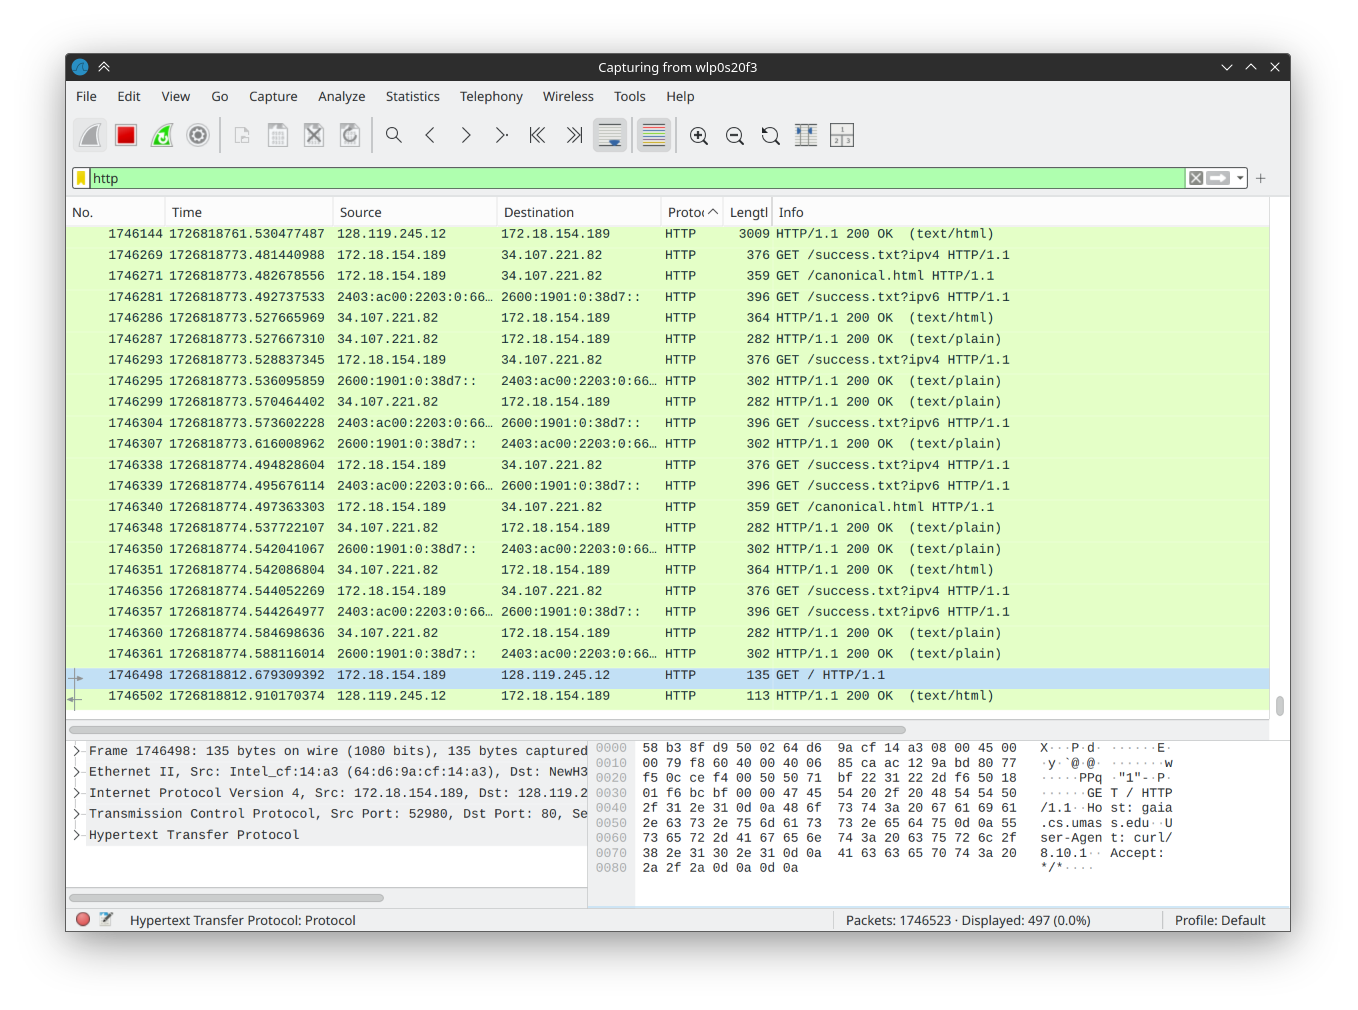
\includegraphics[width=0.8\textwidth]{./lab1-3.png}
    \caption{Internet Address}
    \label{fig:ip}
\end{figure}

We can observe the source and destination columns.

It shows that the source is \texttt{172.18.154.189}, and the destination is \texttt{128.119.245.12}. Therefore, the Internet address of that website is \texttt{128.119.245.12}, and the Internet address of my computer is \texttt{172.18.154.189}, which is a \texttt{LAN} address.

\section*{Problem 4. Print HTTP messages}

\begin{quote}
    Print the two HTTP messages (GET and OK) referred to in question 2 above To do so, select Print from the Wireshark File command menu, and select the
    “Selected Packet Only” and “Print as displayed” radial buttons, and then click OK.
\end{quote}

\subsection*{Solves:}

Follow the instructions, and you will get a menu similar to Fig.~\ref{fig:print}. Press \texttt{OK} to confirm the operation.

\begin{figure}[htbp]
    \centering
    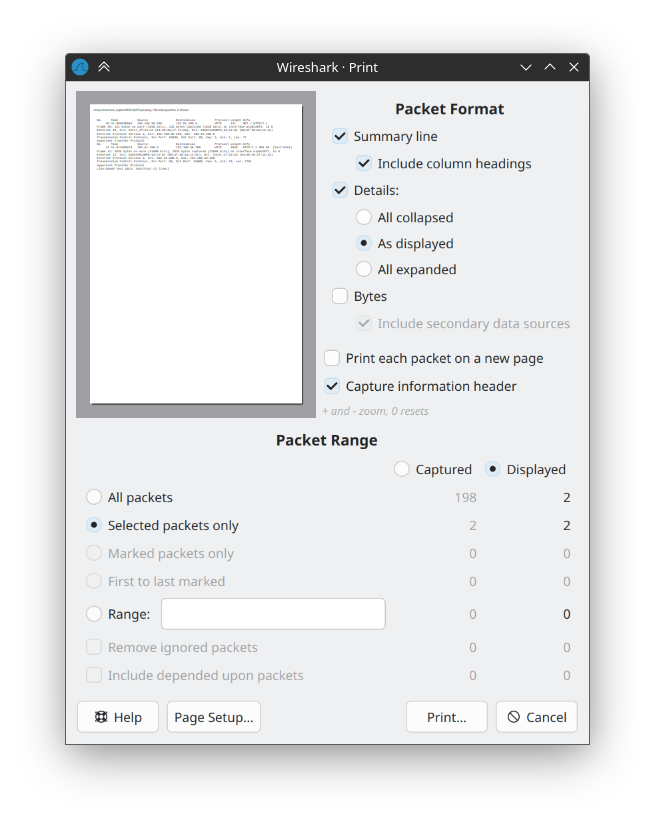
\includegraphics[width=0.68\textwidth]{./lab1-4.png}
    \caption{Print HTTP messages}
    \label{fig:print}
\end{figure}

And choose \texttt{Print to PDF} as the printer. This will generate a PDF file as shown in Fig.~\ref{fig:pdf}."
\begin{figure}[htbp]
    \centering
    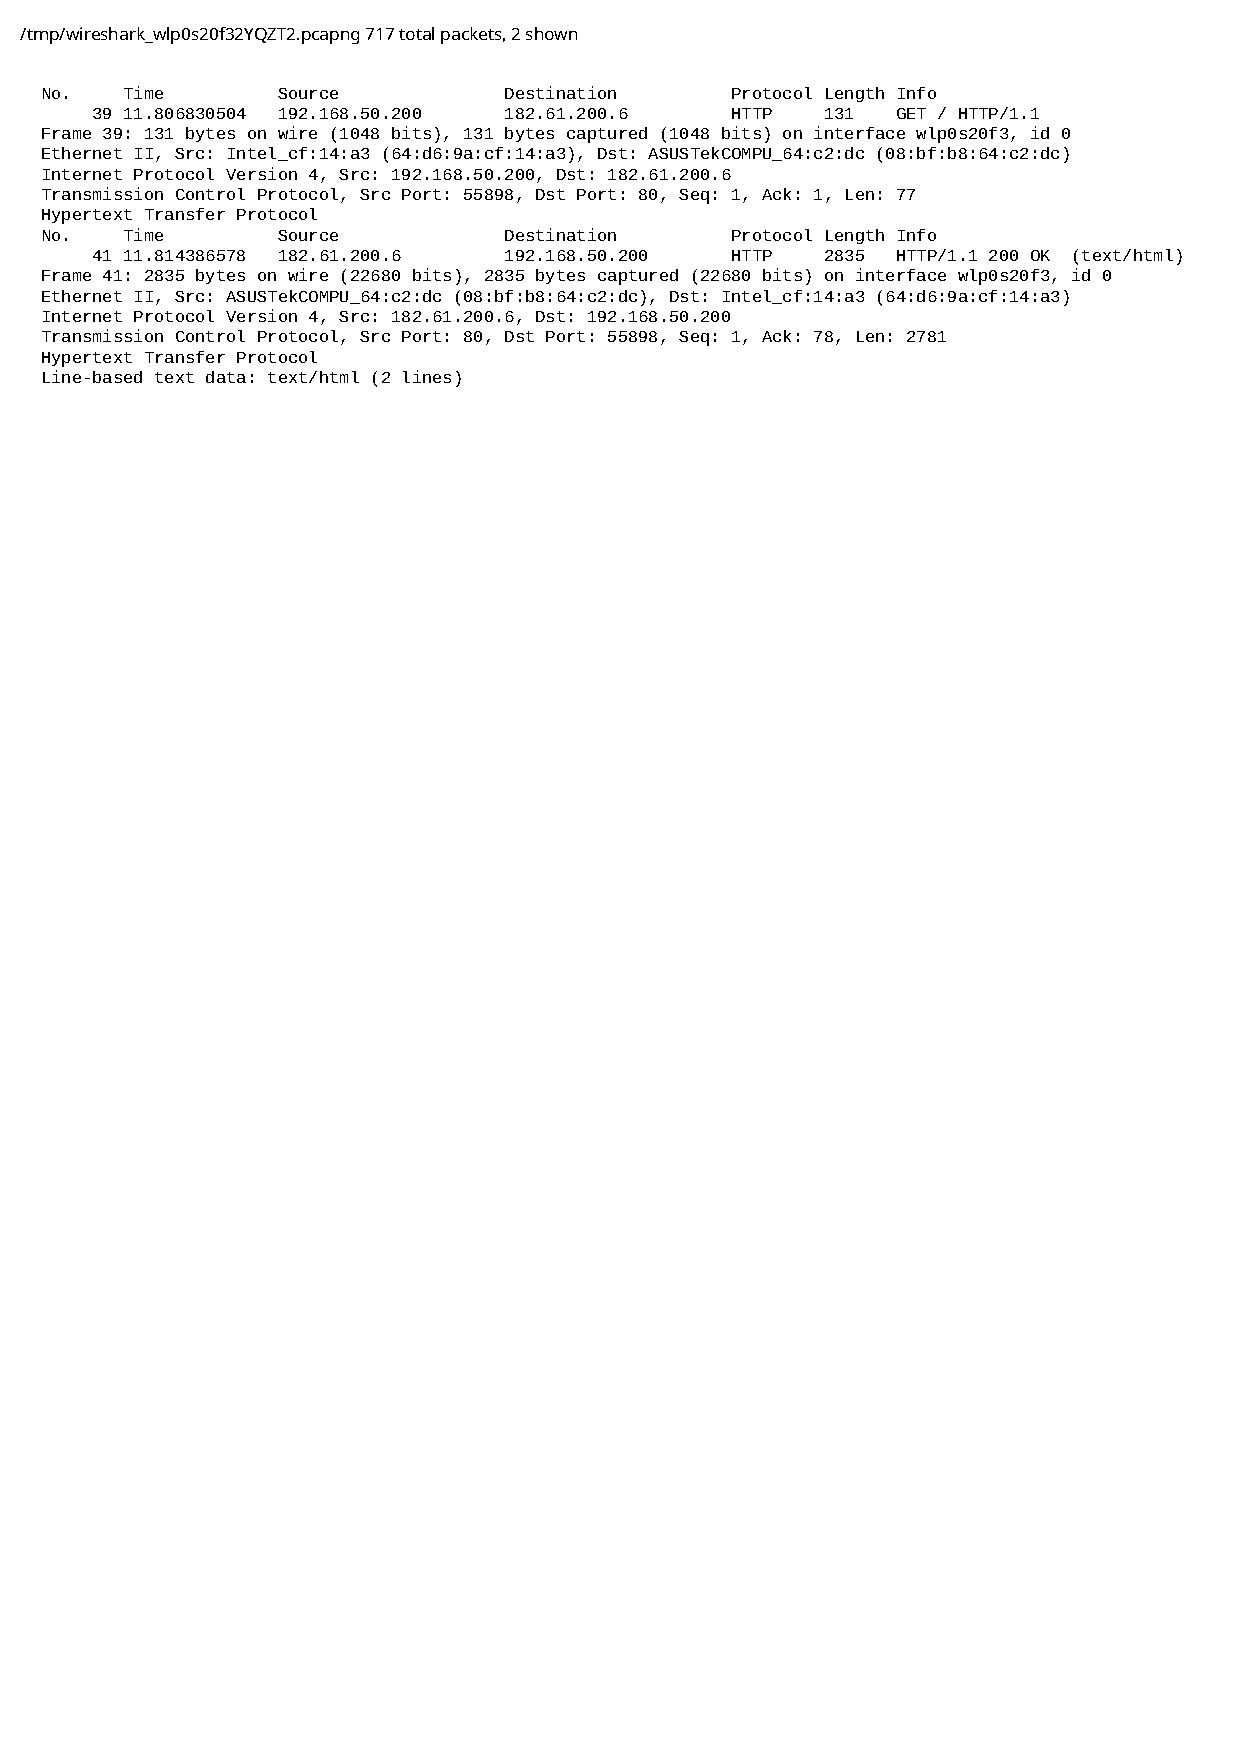
\includegraphics[width=0.7\textwidth]{./lab1-5.pdf}
    \caption{Print Result}
    \label{fig:pdf}
\end{figure}

\end{document}